\section{Exercise 2: Vandermonde Matrix}

In this section we look at exercise 2, which is about Vandermonde matrices. The full script is presented below, and the parts of it specific to subquestions will be discussed in appropriate subsections.

Our script is given by:
\lstinputlisting[language=Python]{Vandermonde.py}

\subsection{2a: fitting by LU decomposition}
The relevant code is given by:
\lstinputlisting[language=Python,firstline=4, lastline=69]{Vandermonde.py}

We start by reading in the data points and constructing the $N \times N$ Vandermonde matrix with each entry of the form $V_{ij} = x_i^j $, with $i$ the row index and $j$ the column index (both up to $N-1$). We then find the coefficients for the unique polynomial that goes through all given points by solving the system $\mathbf{Vc} = \mathbf{y}$ with y the given y-values for the points. 

To do this, we overwrite the Vandermonde matrix by its LU decomposition using Crout's algorithm. We then solve the system by applying forward substitution, followed by backward substitution. 

The result is the unique polynomial given in figure \ref{fig:2a}. 

\begin{figure}[h!]
\label{fig:2a}
\caption{Upper half: the given points in blue, with the polynomial interpolation using LU decomposition in orange. Bottom half: the absolute difference between the interpolation and the given y value at the given points.}
\centering
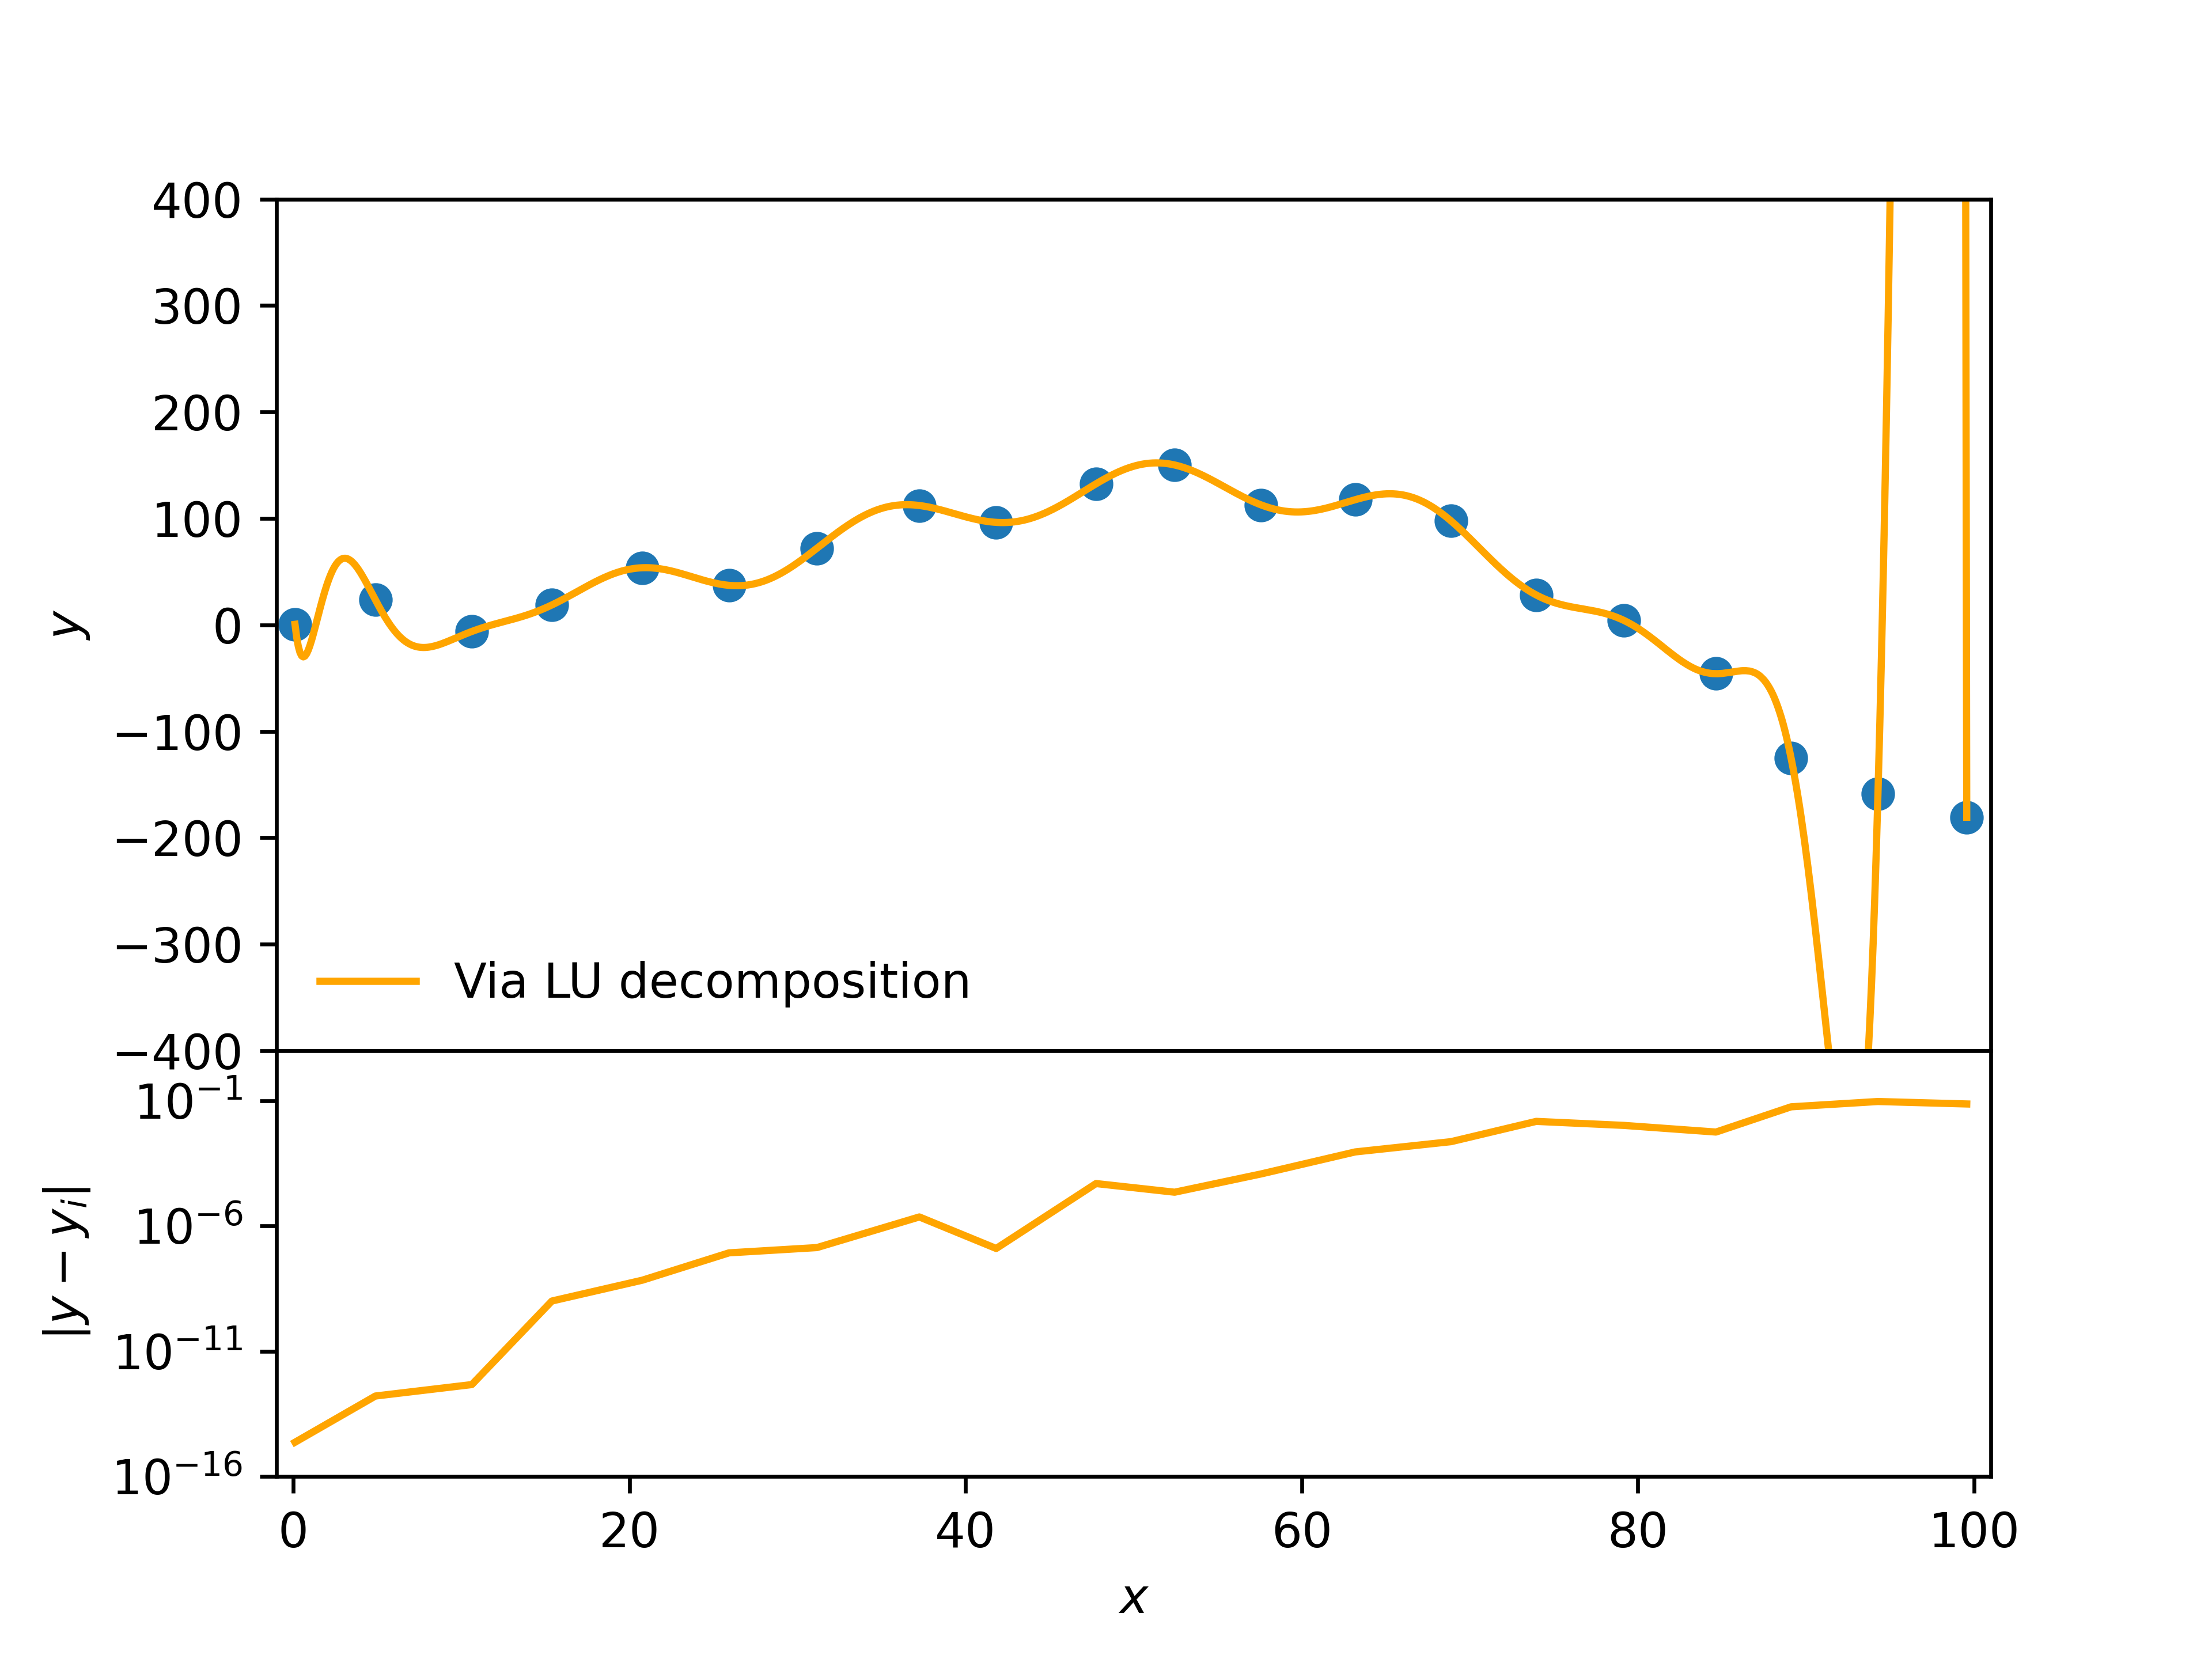
\includegraphics[width=0.6\textwidth]{my_vandermonde_sol_2a.png}
\end{figure}

\lstinputlisting[firstline = 1, lastline = 6]{Vandermonde_output.txt}

\subsection{2b: fitting by Neville's algorithm}
The relevant code is given by:
\lstinputlisting[language=Python,firstline = 70, lastline = 89]{Vandermonde.py}

Here, we simply pass an array of values to be interpolated into our Neville interpolation function. The resulting polynomial lies on top of the polynomial found in 2a. This is to be expected, as there is a single unique 19th order polynomial that goes through all of these points. See figure \ref{fig:2b} below:

\begin{figure}[h!]
\label{fig:2b}
\caption{Upper half: the given points in blue, with the polynomial interpolation using LU decomposition in orange. The polynomial found by Neville's algorithm has been added, and we see that it lies on top of the previous one. Bottom half: the absolute difference between the interpolation and the given y value at the given points. The absolute difference for the second method is orders of magnitude smaller.}
\centering
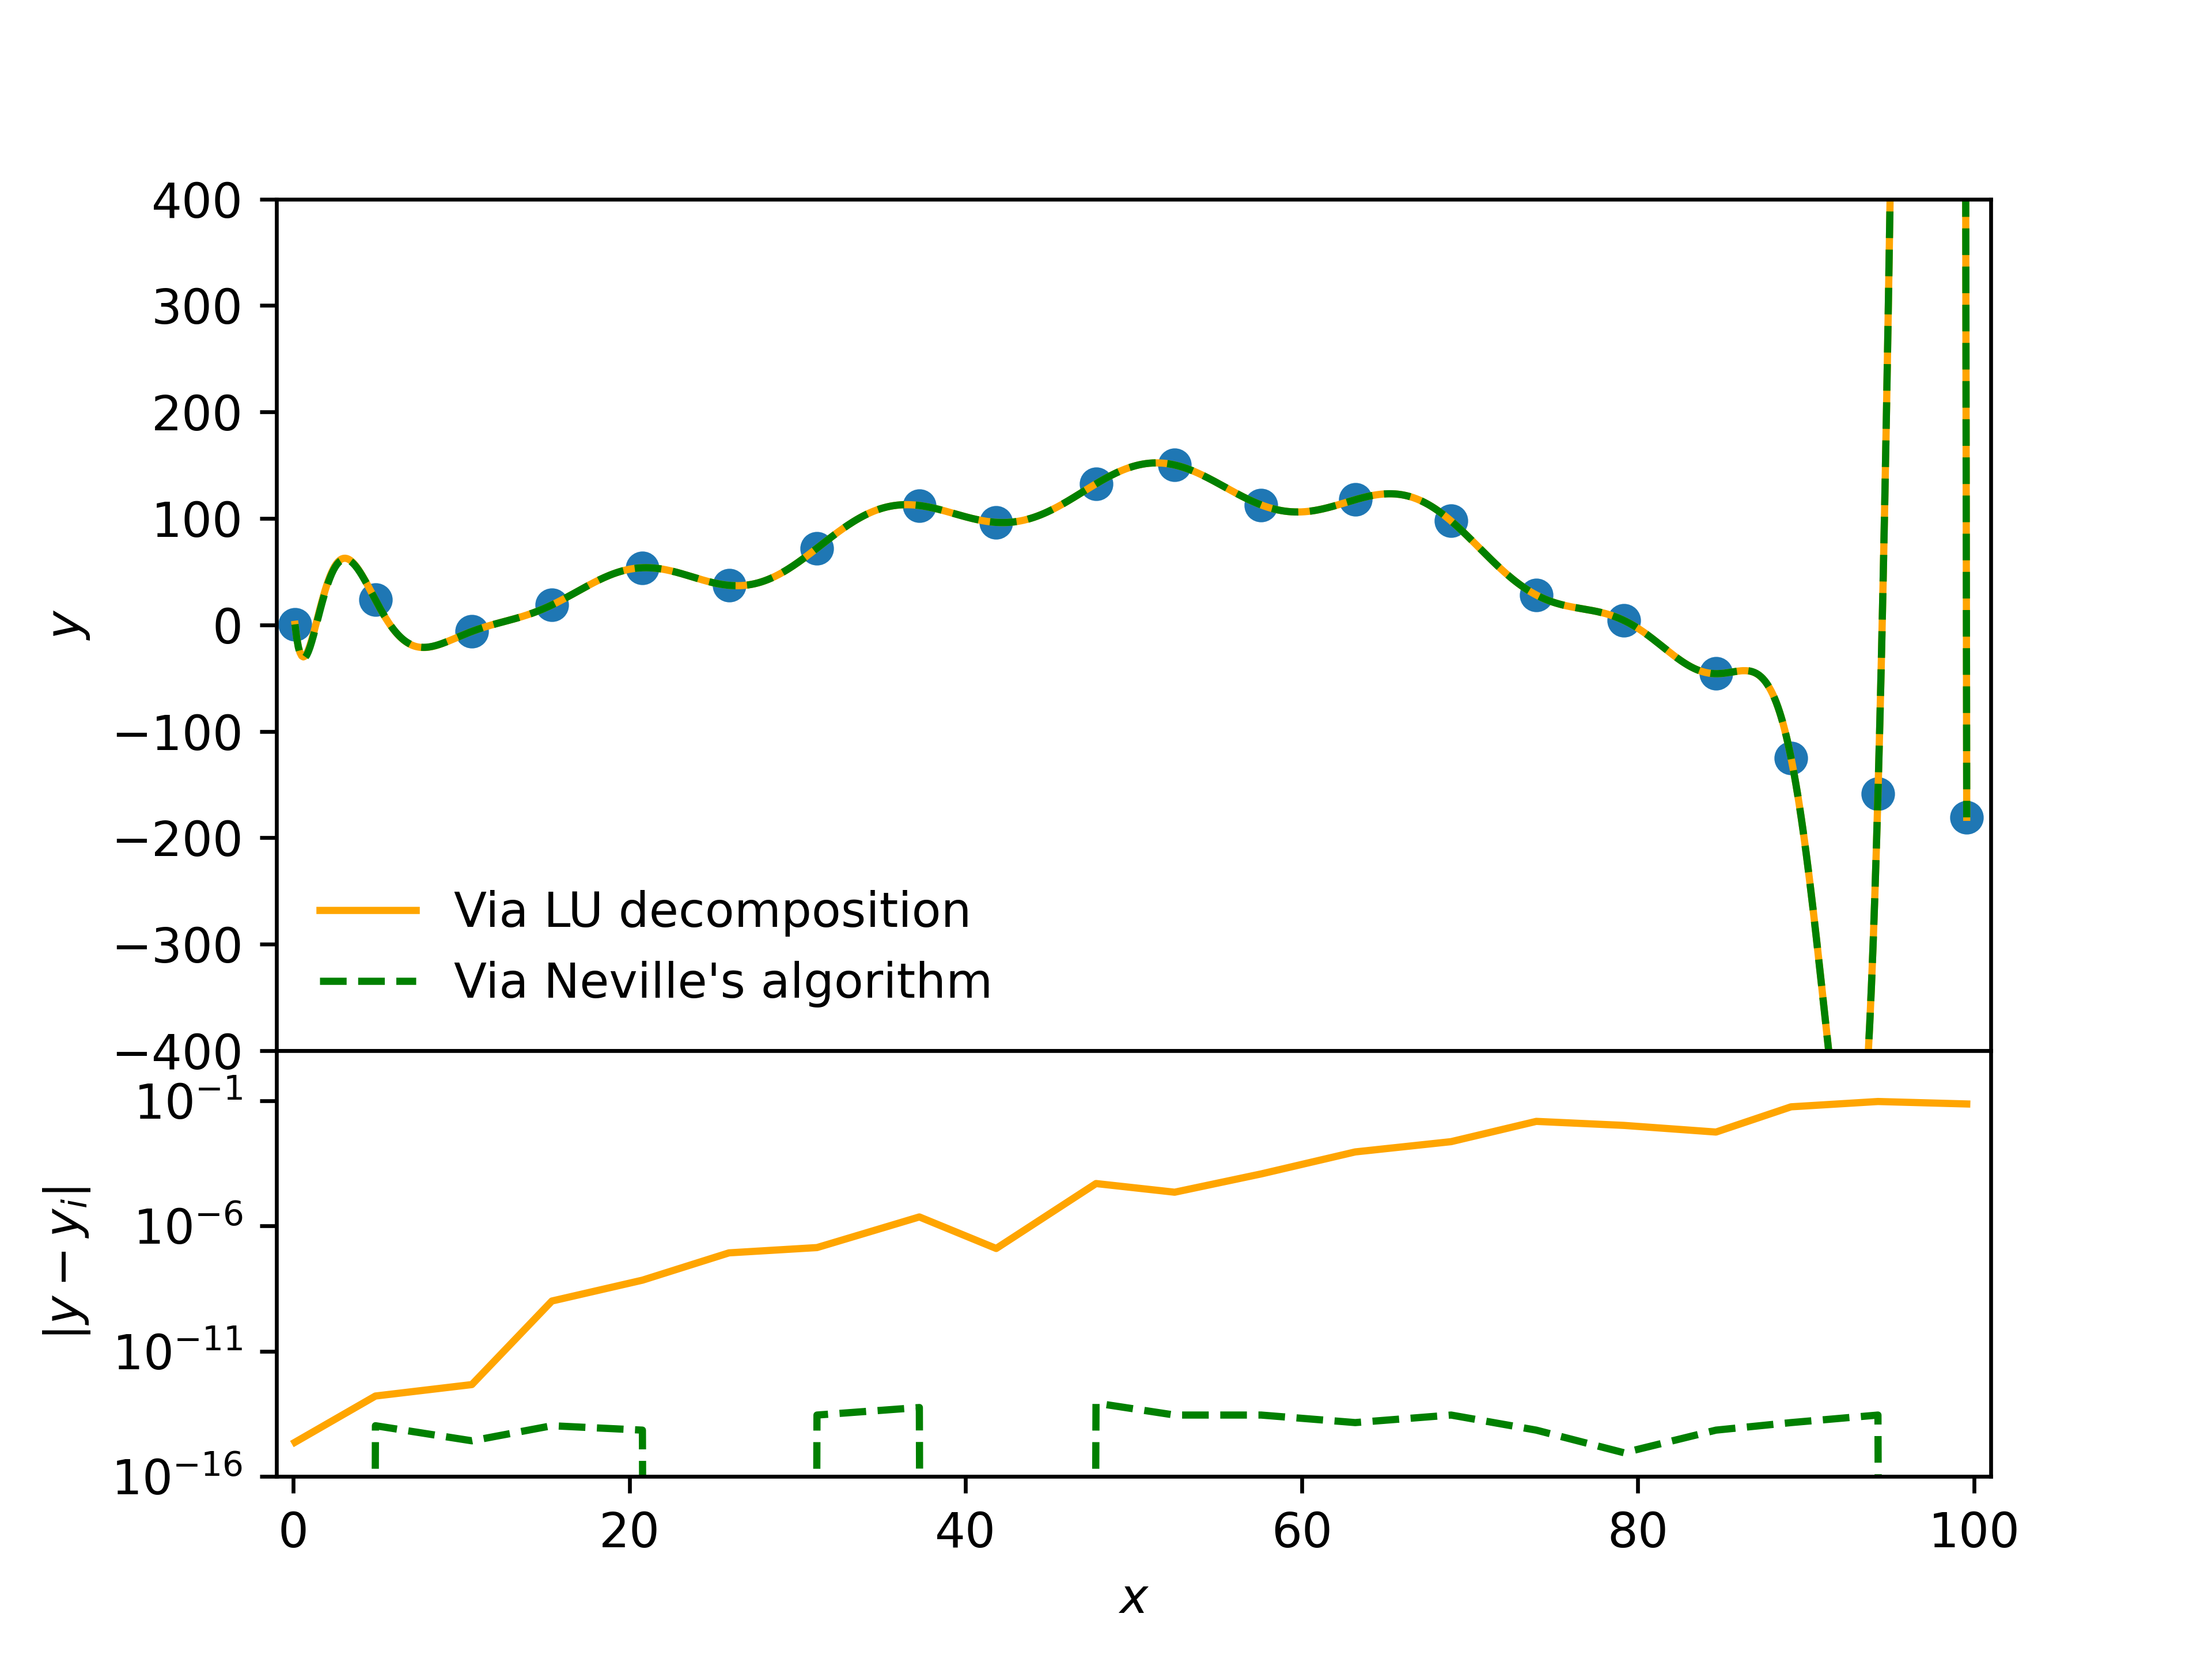
\includegraphics[width=0.6\textwidth]{my_vandermonde_sol_2b.png}
\end{figure}

\lstinputlisting[firstline = 7, lastline = 12]{Vandermonde_output.txt}

Possible reasons for the difference in error are discussed further on in this document.

\subsection{2c: error-cancellation using LU decomposition}
The relevant code is given by:
\lstinputlisting[language=Python,firstline = 90, lastline = 108]{Vandermonde.py}

We now iterate on the solution of 2a. We can use the LU matrices calculated previously and solve a new system to find a correction on the coefficients. We do this once with 1 iteration, and then once more with 10 iterations of the error-cancelling algorithm. The results are shown in figure \ref{fig:2c}.

\begin{figure}[h!]
\label{fig:2c}
\caption{Upper half: the given points in blue, with the polynomial interpolation using LU decomposition in orange, as well as the polynomial found by Neville's algorithm. We have now added 2 additional interpolations, for different iterations of the LU error canceling algorithm. Bottom half: the absolute difference between the interpolation and the given y value at the given points. The absolute difference for the second method is orders of magnitude smaller. The error-canceled LU interpolations are very similar to the initial LU interpolation.}
\centering
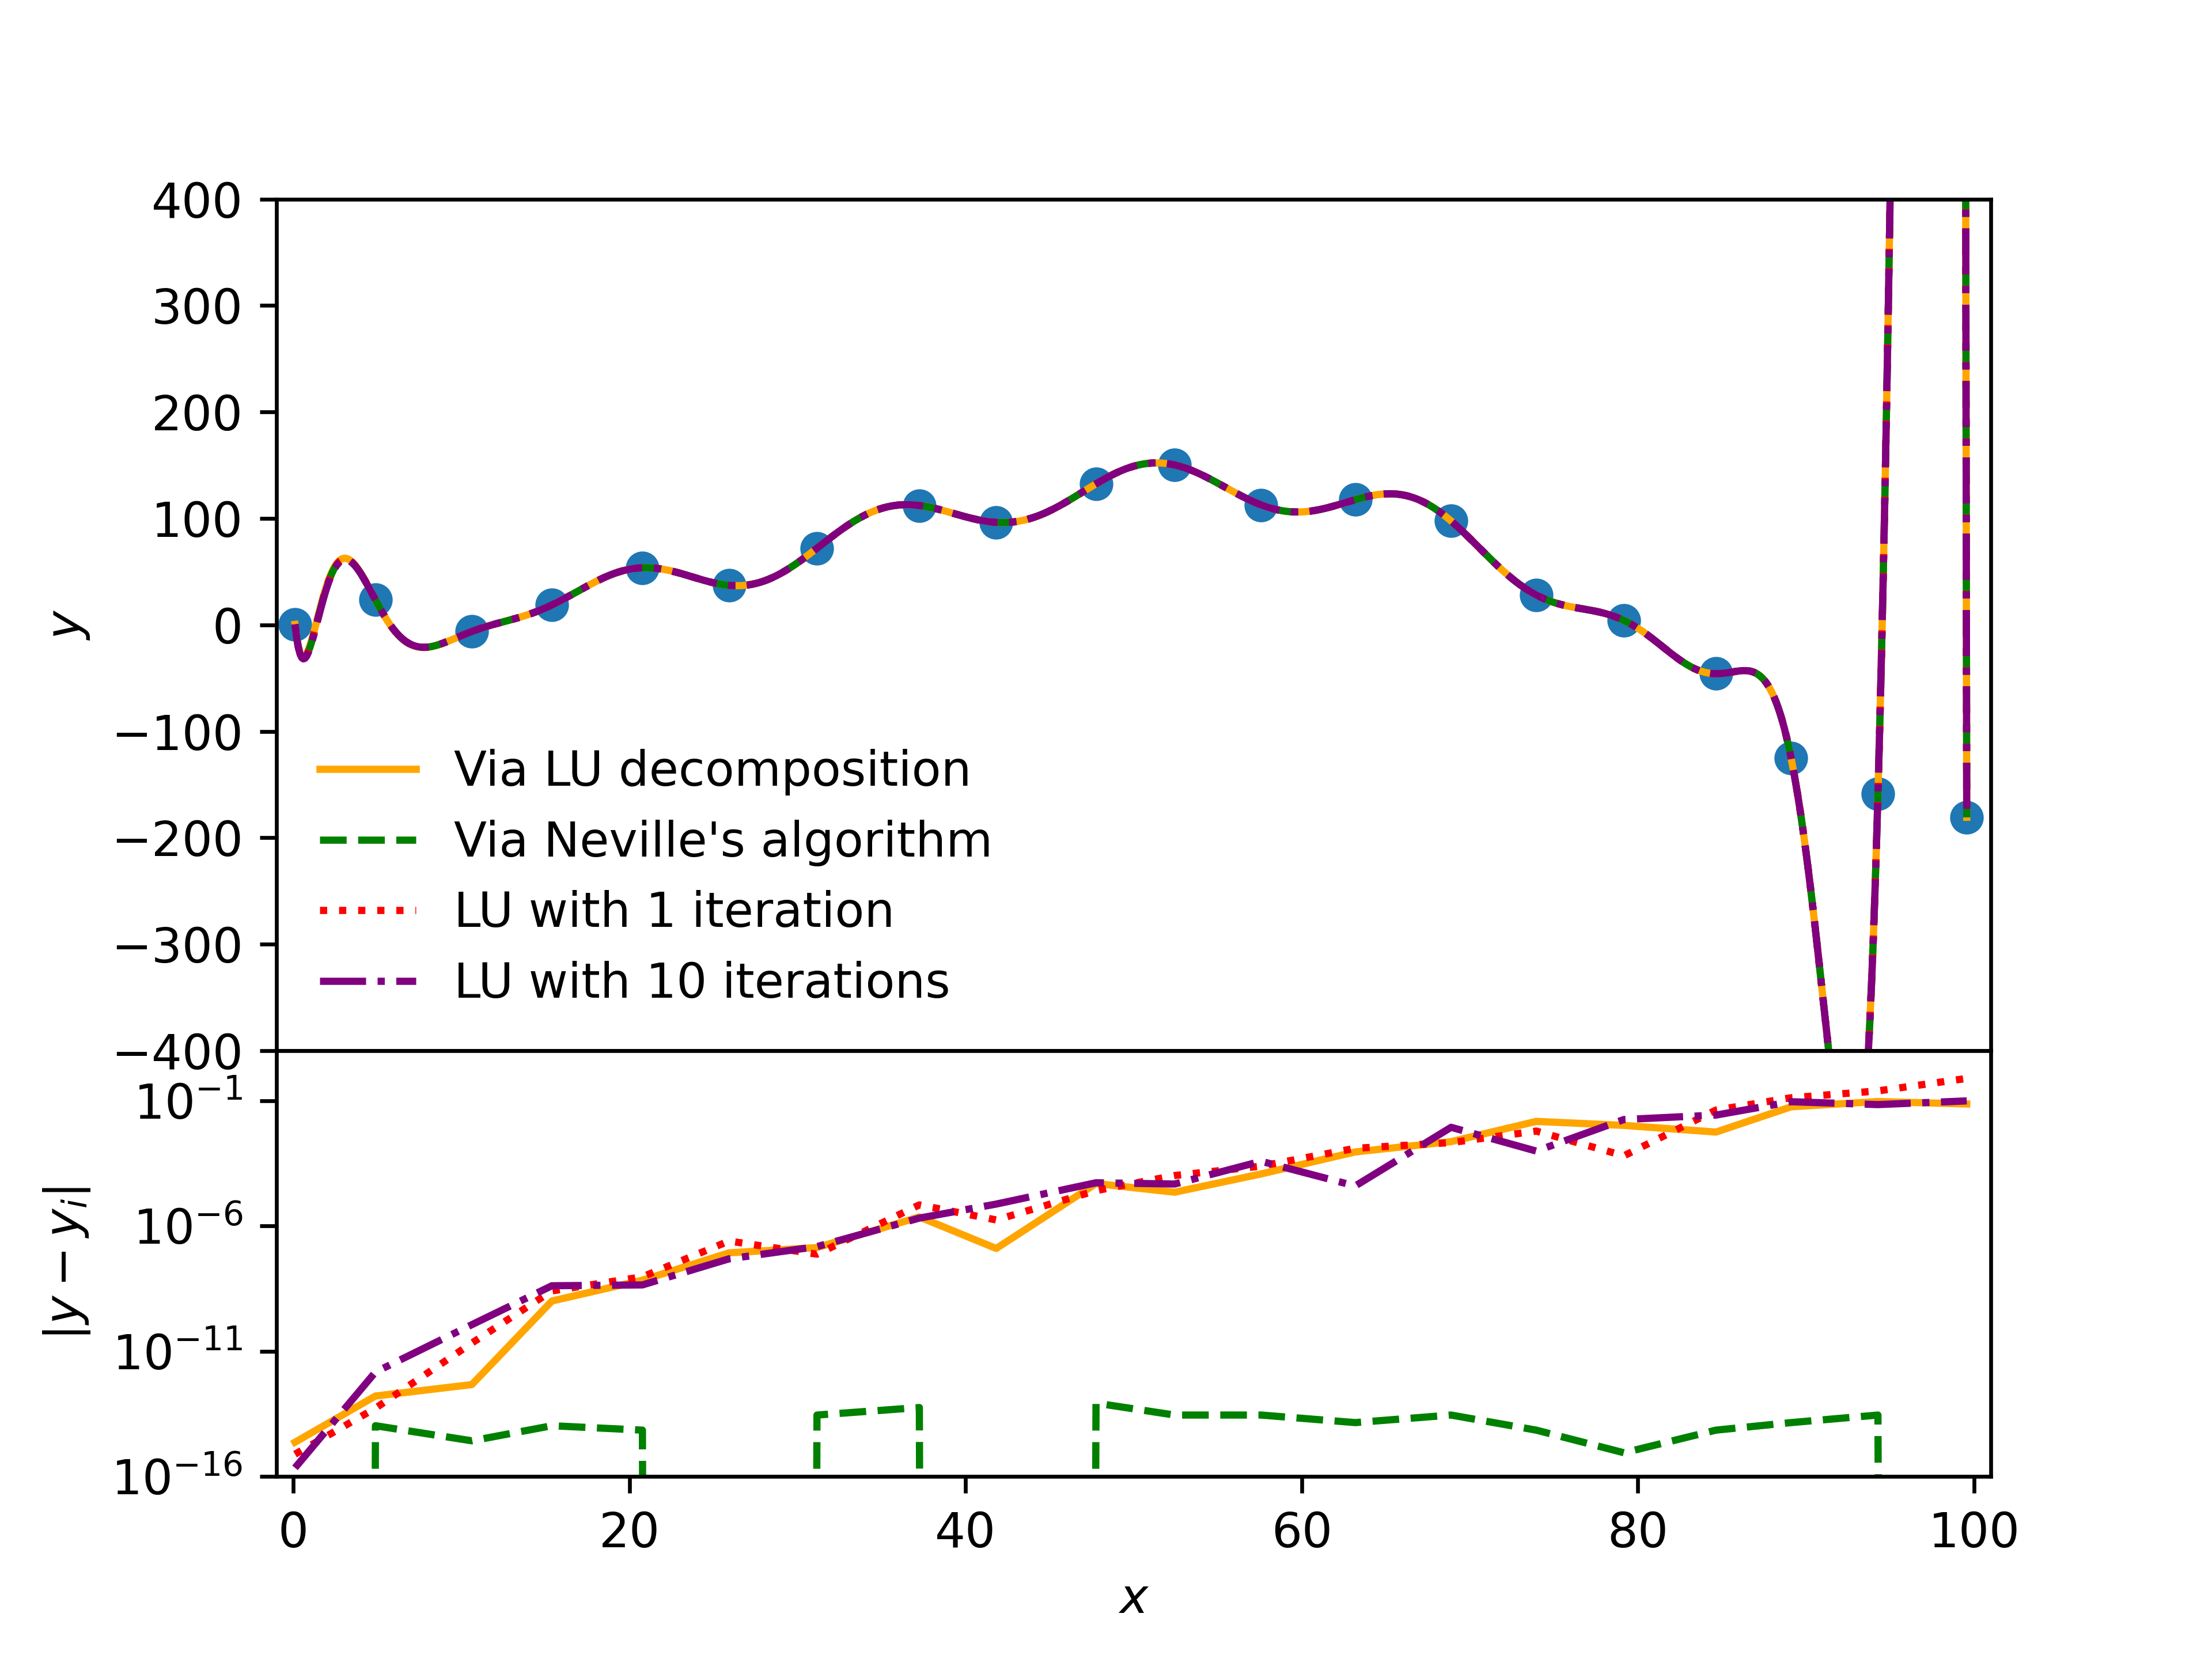
\includegraphics[width=0.6\textwidth]{my_vandermonde_sol_2c.png}
\end{figure}

\lstinputlisting[firstline = 13, lastline = 18]{Vandermonde_output.txt}

\subsection{2d: Timing the interpolation}

Using the timeit module, we execute the code from 2a, 2b and 2c 150 times each. The results are given below:

\lstinputlisting[firstline = 19, lastline = 21]{Vandermonde_output.txt}

We see that the LU decomposition method is quite quick, and the error cancelling doesn't add that much more time. Neville's algorithm is the clear loser when it comes to efficiency. When we take into account accuracy, though, it becomes apparent that Neville's algorithm does have significantly lower errors in this application. A possible cause for error with the LU decomposition method is roundoff. 

We also see that iteration on the LU method takes a small amount of extra time compared to the un-corrected LU method. We also see little to no improvement in error. It is probably the case that, given our implementation of the LU decomposition, we are already at the lowest possible error achievable by that method, and as such we have little to gain with the error cancelling algorithm. 



